\subsection{Is k-cleared-cells NP-hard?}
\label{sub:nphard}

We prove that k-cleared-cells is NP-hard by constructing a reduction from the \textit{Subset sum} problem. The reduction consists of two parts: one part which considers $K > 1$ in the given \textit{Subset sum} instance, and one part which considers the special case $K = 1$. The first part is quite complex and consists of five phases, whereas the second part is relatively straightforward.

The goal of each part is to prove the following: 

\begin{quote}
Given a \textit{Subset sum} instance $Q = \{q_1, \ldots, q_a\}, K \in \mathbb{N}$ there exists a solution $S = \{s_1, \ldots, s_b \} \subseteq Q, \sum S = K$ if and only if there exists a trajectory sequence $\phi$ which clears at least $k$ cells in game $G$ in some instance of \textit{k-cleared-cells}.
\end{quote}

For the general case $K > 1$, we set $k = 8a + 5 \sum Q + 4 + 4K$. For the special case $K = 1$, we set $k = 4$. The block states $P_i$ in $G$ are determined from $Q$ and $K$. This transformation is described in detail in later sections. 

\subsubsection{The initial gameboard}

The initial gameboard $B_0$ in the constructed \textit{k-cleared-cells} instance is pictured in~\autoref{fig:initial}. It consists of two identical structures which will from here on be referred to as \textit{wells}. From the figure we can deduce that $B$ is a $2 \left( \sum Q + K + 1 \right) \times 10$-sized gameboard.

\begin{figure}[H]
    \centering
    \resizebox{0.5\textwidth}{!}{
    \begin{tikzpicture}
        \welldefault{0}{0}
        \welldefault{5}{0}
        \draw[dashed] (0, -1) -- (0, 13);
        \draw[dashed] (10, -1) -- (10, 13);
        \draw[dashed] (-1, 0) -- (11, 0);
        \draw[dashed] (-1, 12) -- (11, 12);
        \draw [decorate,decoration={brace,amplitude=10pt},xshift=-12pt,yshift=0pt]
        (0, 0) -- (0, 10) node [left, black,midway,xshift=-0.5cm]
        {\Huge $2 \left( \sum Q + K \right)$ rows};
        \draw [decorate,decoration={brace,amplitude=10pt},xshift=-12pt,yshift=0pt]
        (0, 10) -- (0, 12) node [left, black,midway,xshift=-0.5cm]
        {\Huge 2 rows};
        \draw [decorate,decoration={brace,amplitude=10pt,mirror},xshift=0pt,yshift=-12pt]
        (0, 0) -- (9, 0) node [below,black,midway,yshift=-0.5cm]
        {\Huge $10$ columns};
    \end{tikzpicture}
    }
    \caption{The initial gameboard}
    \label{fig:initial}
\end{figure}

A schematic of the well structure is pictured in~\autoref{fig:wells}. Please note that the two top rows, denoted \textit{initial block section}, will from here on not be considered part of the well for sake of simplicity. Column 5 of the well is always empty, the content in the other columns depends on which section the rows are in. A well is divided into the following three sections:

\begin{itemize}
\item The bottom section consists of rows in the interval $\left[ 1, 2 \left( K+1 \right) \right]$. In this section, column 1 is alternating white-black, column 2 is alternating black-white, column 3 is white, and column 4 is black.

\item The middle section consists of rows in the interval $\left[ 2 \left( K+1 \right) +1, 2 \left( K-1 + \sum Q \right) \right]$. In this section, column 1 is alternating white-black, column 2 is alternating black-white, column 3 is alternating white-black and column 4 is black.

\item The top section consists of the rows in the interval $\left[2 \left( K-1 + \sum Q \right) +1, 2 \left( K + \sum Q \right) \right]$. In this section columns 2 and 3 are empty. Column 1 consists of white cell in the bottom row, and one white cell in the top row. Column 4 consists of two white cells.

\end{itemize}

\begin{figure}[H]
    \centering
    \resizebox{!}{0.3\paperheight}{
    \begin{tikzpicture}
        \welldetailed{0}{0}
        \draw[dashed] (-1, 0) -- (6, 0);
        \draw[dashed] (-1, 14) -- (6, 14);
        \draw[dashed] (-1, 16) -- (6, 16);
        \draw[dashed] (-1, 18) -- (6, 18);
        \draw[dashed] (-1, 6) -- (6, 6);
        \draw[dashed] (5, 0) -- (5, 18);
        \node at (0.5, -0.5) {\large 1};
        \node at (1.5, -0.5) {\large 2};
        \node at (2.5, -0.5) {\large 3};
        \node at (3.5, -0.5) {\large 4};
        \node at (4.5, -0.5) {\large 5};
        \draw [decorate,decoration={brace,amplitude=10pt},xshift=-12pt,yshift=0pt]
        (0, 0) -- (0, 6) node [left,align=right,black,midway,xshift=-1cm]
        {\huge Bottom section \\ \\
         \huge $2 \left( K-1 \right)$ rows};
        \draw [decorate,decoration={brace,amplitude=10pt},xshift=-12pt,yshift=0pt]
        (0, 6) -- (0, 14) node [left, align=right,black,midway,xshift=-1cm]
        {\huge Middle section \\ \\
         \huge $2 \sum Q$ rows};
        \draw [decorate,decoration={brace,amplitude=10pt},xshift=-12pt,yshift=0pt]
        (0, 14) -- (0, 16) node [left, align=right,black,midway,xshift=-1cm]
        {\huge Top section};
        \draw [decorate,decoration={brace,amplitude=10pt},xshift=-12pt,yshift=0pt]
        (0, 16) -- (0, 18) node [left, align=right,black,midway,xshift=-1cm]
        {\huge Initial block section};
        \draw (3.5, 0.5) -- (7, 0.5) node [right, black, xshift=1cm] 
        {\huge row 1};
        \draw (3.5, 6.5) -- (7, 6.5) node [right, black, xshift=1cm, yshift=-1.5cm]
        {\huge row $2 \left( K-1 \right)$};
        \draw (3.5, 5.5) -- (7, 5.5) node [right, black, xshift=1cm, yshift=1.5cm]
        {\huge row $2 \left( K-1 \right) +1$};
        \draw (3.5, 13.5) -- (7, 13.5) node [right, black, xshift=1cm]
        {\huge row $2 \left( K-1+ \sum Q \right)$};
    \end{tikzpicture}
    }
    \caption{The well structure}
    \label{fig:wells}
\end{figure}

The purpose of the well is to force the placement of blocks in play. One feature of the well structure is that if we were to drop a block with 2 black cells on the right half in column 4-5, the black right half would drop down and instantly clear itself and the two bottommost cells in column 4. The terrain in column 4 would then collapse, making place for a new block to be placed in the same manner.

This feature cannot be utilized in the default well state though, since fixing a block on the top of column 5 would result in a losing state. Would the two right white cells in the top section disappear, this feature becomes available. This characteristic of the well is heavily used in this reduction. We therefore provide three definitions regarding this to aid in the proof. If the well is \textit{closed}, placing a block in column 4-5 yields a game over, if the well is \textit{open} this placement does not yield a game over. If a game is \textit{blocked}, the no blocks can be place anywhere in the well without yielding a losing state. If a well is blocked, it is also impossible to unblock it during the game. The appearances of the top section for all open and closed well states is the ones depicted in in~\autoref{fig:openclosed}. The appearance of the top section in a blocked well may however appear differently. The reason for this will later become apparent.

\begin{figure}[H]
    \centering
    \begin{subfigure}[b]{0.15\linewidth}
        \resizebox{\linewidth}{!}{
            \begin{tikzpicture}
                \topclosed{0}{0}
            \end{tikzpicture}
        }
        \caption{Closed}
    \end{subfigure}
    \hspace{0.02\linewidth}
    \begin{subfigure}[b]{0.15\linewidth}
        \resizebox{\linewidth}{!}{
            \begin{tikzpicture}
                \topopen{0}{0}
            \end{tikzpicture}
        }
        \caption{Open}
    \end{subfigure}
    \hspace{0.02\linewidth}
    \begin{subfigure}[b]{0.15\linewidth}
        \resizebox{\linewidth}{!}{
            \begin{tikzpicture}
                \topclosed{0}{0}
                \lumx{1}{6}
            \end{tikzpicture}
        }
        \caption{Blocked}
    \end{subfigure}
    \caption{Open and closed wells}
    \label{fig:openclosed}
\end{figure}

The following lemma will be used during the whole reduction and explains an important property of the terrain we use in the initial gameboard.\\

\begin{lem}
\label{lem:alternatingrows}
A column with an interval of alternating rows may only have its top or bottom cell cleared. This is only possible if there is a cell in the same column which is both the same color as one of these cells and adjacent to it.
\end{lem}

\begin{proof}
In \ref{subsub:gameplay} it is defined that for a cell to be marked and cleared its surrounding cells must be the same color. If a column has an interval of alternating rows we know that there are no two adjecent cells with the same color in that interval. Therefore the only way a cell part of the interval can be cleared is if it is directly below or above a cell not part of the interval. This leaves the top and bottom cell the only possibilities.
\end{proof}


The following lemma will be used during the whole reduction and explains an important property of the terrain we use in the initial gameboard.\\

\begin{lem}
\label{lem:alternatingrows}
A column with an interval of alternating rows may only clear the top or bottom cell. This is only possible if there is a cell in the column not part of the interval with the same color adjacent to the bottom respectively the top cell.
\end{lem}

\begin{proof}
In \ref{subsub:gameplay} it is defined that for a cell to be marked and cleared its surrounding cells must be the same color. If a column has an interval of alternating rows we know that there are no two adjecent cells with the same color in the column. Therefore the only way a cell part of the interval can be cleared is if it is adjecent to a cell not part of the interval. This leaves only the top and bottom cell.
\end{proof}

\subsubsection{Phase 1}
In this phase we transform every $q_i \in Q$ to sequences of game blocks. These sequences will be part of the block states $P_1, \ldots P_n$ in the constructed \textit{k-cleared-cells} instance. The transformation is done by creating a sequence of 1 $\mathbf{H}_{H}$, $q_i$ $\mathbf{H}$ and 1 $\mathbf{H}_H$ blocks (in their initial state) for each give $q_i$.

\begin{figure}[H]
    \centering
    \resizebox{0.4\textwidth}{!}{
    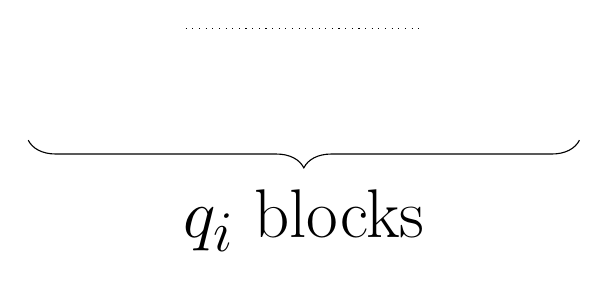
\begin{tikzpicture}
        \startb{0}{0}
        \middleb{3}{0}
        \draw[dotted] (5, 1) -- (8, 1);
        \middleb{8}{0}
        \startb{11}{0}
        \draw [decorate,decoration={brace,amplitude=10pt,mirror},xshift=0pt,yshift=-12pt]
        (3, 0) -- (10, 0) node [below,black,midway,yshift=-0.5cm]
        {\Huge $q_i$ blocks};
    \end{tikzpicture}
    }
    \caption{Transformation of \textit{Subset sum} element $q_i$}
    \label{fig:wells}
\end{figure}

When placing the first block it is evident that we have only two choices: place the $\mathbf{H}_H$ block column 2-3 of any well. This transform the chosen well from a closed to an open state. We then proceed to placing the middle $q_i$ blocks. When deciding the outcome of these placements the following lemmas are of use:\\

\begin{lem}
TODO: prove that the height doesn't change in the columns in phase 1. Important for second lemma.
\end{lem}

\bigbreak

\begin{lem}
\label{lem:permclose}
In phase 1, placing a $\mathbf{H}$ block in any other column than 4-5 in a well will make the same well permanently closed.
\end{lem}

\begin{proof}
In the first case, the well is closed. We can only place the $\mathbf{H}$ block in column 2-3. Since no cells are cleared as a result, column 1 to 4 are filled except for the top two rows. We therefore cannot place any block in these columns without a game over. Either the column right of column 5 is filled, or the gameboard has ended. Since column 4 is also filled, we cannot place any block in column 5. Thus the well is permanently closed.

In the second case, the well is open. Apart from column 4-5, the $\mathbf{H}$ block can only be placed in column 3-4. This does not clear any cells as a result. Thus with the same arguments as in the first case, the well is permanently closed.
\end{proof}

Since later in the proof it will become apparent that having a permanently closed well makes it impossible to construct a optimal trajectory sequence, lemma~\ref{lem:permclose} leaves us no choice but to place all $\mathbf{H}$ blocks in column 4-5 of the open well. Finally the last $\mathbf{H}_H$ block must be placed either in column 2-3 of a closed well, or column 3-4 of an open well, in order to not permanently close a well.

\begin{figure}[H]
    \centering
    \begin{subfigure}[b]{0.55\textwidth}
        \resizebox{\linewidth}{!}{
            \begin{tikzpicture}
                \welldefault{0}{0}
                \startb{1}{10}
                \welldefault{5}{0}
                \draw[dashed] (0, 0) -- (0, 12);
                \draw[dashed] (10, 0) -- (10, 12);
                \draw[dashed] (0, 0) -- (10, 0);
                \draw[->, line width=10pt] (11, 6) -- (14, 6);
                \wellopenwhole{15}{0}
                \welldefault{20}{0}
                \draw[dashed] (15, 0) -- (15, 12);
                \draw[dashed] (25, 0) -- (25, 12);
                \draw[dashed] (15, 0) -- (25, 0);
            \end{tikzpicture}
        }
        \caption{First block}
    \end{subfigure}

    \begin{subfigure}[b]{0.55\textwidth}
        \resizebox{\linewidth}{!}{
            \begin{tikzpicture}
                \wellopenwhole{0}{0}
                \middleb{3}{10}
                \welldefault{5}{0}
                \draw[dashed] (0, 0) -- (0, 12);
                \draw[dashed] (10, 0) -- (10, 12);
                \draw[dashed] (0, 0) -- (10, 0);
                \draw[->, line width=10pt] (11, 6) -- (14, 6);
                \wellopenwhole{15}{0}
                \cellw{18}{7}
                \cellw{18}{6}
                \welldefault{20}{0}
                \draw[dashed] (15, 0) -- (15, 12);
                \draw[dashed] (25, 0) -- (25, 12);
                \draw[dashed] (15, 0) -- (25, 0);
            \end{tikzpicture}
        }
        \caption{Middle blocks}
    \end{subfigure}

    \begin{subfigure}[b]{0.55\textwidth}
        \resizebox{\linewidth}{!}{
            \begin{tikzpicture}
                \wellopenwhole{0}{0}
                \cellw{3}{7}
                \cellw{3}{6}
                \startb{2}{10}
                \welldefault{5}{0}
                \draw[dashed] (0, 0) -- (0, 12);
                \draw[dashed] (10, 0) -- (10, 12);
                \draw[dashed] (0, 0) -- (10, 0);
                \node at (12.5, 6)
                {\Huge or};
                \wellopenwhole{15}{0}
                \cellw{18}{7}
                \cellw{18}{6}
                \welldefault{20}{0}
                \startb{21}{10}
                \draw[dashed] (15, 0) -- (15, 12);
                \draw[dashed] (25, 0) -- (25, 12);
                \draw[dashed] (15, 0) -- (25, 0);
            \end{tikzpicture}
        }
        \caption{Final block}
    \end{subfigure}

    \caption{Block placement in phase 1}
    \label{fig:placement}
\end{figure}

Assuming that no blocks has been place such that any well is permanently closed, the following invariants holds at the start of the sequence corresponding to $q_i$:

\begin{enumerate}
\item Either both of the wells are closed, or both of the wells are open.

\item Column 1, 3 and 5 in any well are unchanged from the initial gameboard. Column 2 is unchanged except from the top two rows (which may be black or empty).

\item Let $q_0 = 0$. This does not change the semantics of the givet \textit{Subset sum} instance. Then in total 
\begin{equation*}
    2 \left( i-1 \right) + \sum_{j=0}^{i-1} q_j
\end{equation*}
blocks have been placed.

\item Since each block placement clears exactly 4 cells
\begin{equation*}
    8 \left( i-1 \right) + 4 \sum_{j=0}^{i-1} q_j
\end{equation*}
cells have been cleared.

\item There exists: 
    \begin{equation*}
        M_1, M_2 \subseteq \{q_0, \ldots q_{i-1}\}, M_1 \cap M_2 = \varnothing, M_1 \cup M_2 = \{q_0, \ldots, q_{i-1}\}
    \end{equation*}
such that for any well $w \in \{1,2\}$ it holds that the rows in interval
    \begin{equation*}
        \left[ 2 \left( K-1 + \sum Q - \sum M_w \right) +1, 2 \left( K-1 + \sum Q \right) \right]
    \end{equation*}
consists of white cells in column 4, and the rows in interval
    \begin{equation*}
        \left[ 1, 2 \left( K-1 + \sum Q - \sum M_w \right) \right]
    \end{equation*}
consists of black cells in column 4.
\end{enumerate}

\begin{figure}[H]
    \centering
    \resizebox{!}{0.3\paperheight}{
    \begin{tikzpicture}
        \invariantchart{0}{0}
        \draw[dashed] (-1, 0) -- (6, 0);
        \draw[dashed] (-1, 6) -- (6, 6);
        \draw[dashed] (-1, 12) -- (6, 12);
        \draw[dashed] (-1, 20) -- (6, 20);
        \draw[dashed] (5, 0) -- (5, 22);
        \node at (0.5, -0.5) {\large 1};
        \node at (1.5, -0.5) {\large 2};
        \node at (2.5, -0.5) {\large 3};
        \node at (3.5, -0.5) {\large 4};
        \node at (4.5, -0.5) {\large 5};
        \draw [decorate,decoration={brace,amplitude=10pt},xshift=-12pt,yshift=0pt]
        (0, 0) -- (0, 6) node [left,align=right,black,midway,xshift=-1cm]
        {\huge $2 \left( K-1 \right)$ rows};
        \draw [decorate,decoration={brace,amplitude=10pt},xshift=-12pt,yshift=0pt]
        (0, 6) -- (0, 12) node [left,align=right,black,midway,xshift=-1cm]
        {\huge $2 \left( \sum Q - \sum M_w \right)$ rows};
        \draw [decorate,decoration={brace,amplitude=10pt},xshift=-12pt,yshift=0pt]
        (0, 12) -- (0, 20) node [left,align=right,black,midway,xshift=-1cm]
        {\huge $2 \sum M_w $ rows};
        \draw (3.5, 0.5) -- (7, 0.5) node [right, black, xshift=1cm] 
        {\huge row 1};
        \draw (3.5, 5.5) -- (7, 5.5) node [right, black, xshift=1cm, yshift=-0.5cm] 
        {\huge row $2 \left( K-1 \right)$};
        \draw (3.5, 6.5) -- (7, 6.5) node [right, black, xshift=1cm, yshift=0.5cm] 
        {\huge row $2 \left( K-1 \right) + 1$};
        \draw (3.5, 11.5) -- (7, 11.5) node [right, black, xshift=1cm, yshift=-0.5cm] 
        {\huge row $2 \left( K-1 + \sum Q - \sum M_w \right)$};
        \draw (3.5, 12.5) -- (7, 12.5) node [right, black, xshift=1cm, yshift=0.5cm] 
        {\huge row $2 \left( K-1 + \sum Q - \sum M_w \right) +1$};
        \draw (3.5, 19.5) -- (7, 19.5) node [right, black, xshift=1cm] 
        {\huge row $2 \left( \sum Q + K - 1 \right)$};
    \end{tikzpicture}
    }
    \caption{Depiction of invariants}
    \label{fig:invariant}
\end{figure}

When every block sequence corresponding to the elements of $Q$ has been placed, $a$ elements has been transformed. For all purposes of this proof this is equivalent to being at the start of the sequence corresponding to $q_{a+1}$, even though strictly speaking no such element is given. Thus $i = a+1$ and from the invariants we obtain:

\begin{enumerate}
\item Still holds.
\item Still holds.
\item In total
\begin{equation*}
    2a + \sum Q
\end{equation*}
blocks have been placed.

\item In total
\begin{equation*}
    8a + 4 \sum Q
\end{equation*}
cells have been cleared.

\item There exists:
\begin{equation*}
    M_1, M_2 \subseteq Q, M_1 \cap M_2 = \varnothing, M_1 \cup M_2 = Q
\end{equation*}
such that for any well $w \in \{1,2\}$ it holds that the rows in interval
\begin{equation*}
        \left[ 2 \left( K-1 + \sum Q - \sum M_w \right) +1, 2 \left( K-1 + \sum Q \right) \right]
    \end{equation*}
consists of white cells in column 4, and the rows in interval
    \begin{equation*}
        \left[ 1, 2 \left( K-1 + \sum Q - \sum M_w \right) \right]
    \end{equation*}
consists of black cells in column 4.
\end{enumerate}


\subsubsection{Phase 2}
\label{subsub:phasetwo}
In this phase a single $\mathbf{X}_H$ block is generated. From the invariants presented in~\ref{subsub:phaseone} we know that the top of the two wells must be in one of the two states presented in~\autoref{fig:openclosed}. Thus the only non-losing option is to place the $\mathbf{X}_H$ block in such a way that it closes one of the wells permanently. Note that if any well was permanently closed before this phase, this placement renders both of the wells permanently closed, making it impossible to clear any more cells during the game.

\begin{figure}[H]
    \centering
    \begin{subfigure}[b]{0.35\textwidth}
        \resizebox{\linewidth}{!}{
            \begin{tikzpicture}
            \ptwoclosed{0}{0}
            \stopb{1}{8}
            \draw[dashed] (0, 0) -- (0, 10);
            \draw[dashed] (5, 0) -- (5, 10);
            \draw[->, line width=5pt] (6, 5) -- (9, 5);
            \ptwoclosed{10}{0}
            \draw[dashed] (10, 0) -- (10, 10);
            \draw[dashed] (15, 0) -- (15, 10);
            \stopb{11}{6}
            \end{tikzpicture}
        }
        \caption{}
    \end{subfigure}
    \hspace{0.05\textwidth}
    \begin{subfigure}[b]{0.35\textwidth}
        \resizebox{\linewidth}{!}{
            \begin{tikzpicture}
            \ptwoopen{0}{0}
            \stopb{2}{8}
            \draw[dashed] (0, 0) -- (0, 10);
            \draw[dashed] (5, 0) -- (5, 10);
            \draw[->, line width=5pt] (6, 5) -- (9, 5);
            \ptwoopen{10}{0}
            \stopb{12}{6}
            \draw[dashed] (10, 0) -- (10, 10);
            \draw[dashed] (15, 0) -- (15, 10);
            \end{tikzpicture}
        }
        \caption{}
    \end{subfigure}

    \begin{subfigure}[b]{0.35\textwidth}
        \resizebox{\linewidth}{!}{
            \begin{tikzpicture}
            \ptwoopen{0}{0}
            \stopb{3}{8}
            \draw[dashed] (0, 0) -- (0, 10);
            \draw[dashed] (5, 0) -- (5, 10);
            \draw[->, line width=5pt] (6, 5) -- (9, 5);
            \ptwoopen{10}{0}
            \cellw{13}{6}
            \cellb{13}{7}
            \draw[dashed] (10, 0) -- (10, 10);
            \draw[dashed] (15, 0) -- (15, 10);
            \end{tikzpicture}
        }
        \caption{}
    \end{subfigure}

    \caption{Possible cases in phase 2}
    \label{fig:placement}
\end{figure}


\subsubsection{Phase 3}

In this phase the sequence $\left( \mathbf{MB}, \mathbf{MW}, \mathbf{X} \right)$ is generated. According to the reasoning in~\nameref{subsub:phasetwo} the game must either be in an unplayable state or be in a state such that one well is permanently closed and the other well has the appearance pictured in~\autoref{fig:openclosed}. The well that is not permanently closed can thus be in one of two possible states. For each case there is exactly one way of placing the block sequence such that this well is not also permanently closed. Placing the blocks in this way will clear 10 cells regardless of case.

\begin{figure}[H]
    \centering
    \begin{subfigure}[b]{0.8\textwidth}
        \resizebox{\linewidth}{!}{
            \begin{tikzpicture}
            \ptwoclosed{0}{0}
            \lummonoblack{1}{8}
            \draw[dashed] (0, 0) -- (0, 10);
            \draw[dashed] (5, 0) -- (5, 10);
            \draw[->, line width=5pt] (6, 5) -- (9, 5);
            \ptwoclosed{10}{0}
            \draw[dashed] (10, 0) -- (10, 10);
            \draw[dashed] (15, 0) -- (15, 10);
            \lummonowhite{11}{8}
            \draw[->, line width=5pt] (16, 5) -- (19, 5);
            \pthreeone{20}{0}
            \stopb{21}{8}
            \draw[dashed] (20, 0) -- (20, 10);
            \draw[dashed] (25, 0) -- (25, 10);
            \end{tikzpicture}
        }
        \caption{}
        \vspace*{1cm}
    \end{subfigure}

    \begin{subfigure}[b]{0.8\textwidth}
        \resizebox{\linewidth}{!}{
            \begin{tikzpicture}
            \ptwoopen{0}{0}
            \lummonoblack{2}{8}
            \draw[dashed] (0, 0) -- (0, 10);
            \draw[dashed] (5, 0) -- (5, 10);
            \draw[->, line width=5pt] (6, 5) -- (9, 5);
            \pthreeone{10}{0}
            \draw[dashed] (10, 0) -- (10, 10);
            \draw[dashed] (15, 0) -- (15, 10);
            \lummonowhite{11}{8}
            \draw[->, line width=5pt] (16, 5) -- (19, 5);
            \pthreeone{20}{0}
            \stopb{21}{8}
            \draw[dashed] (20, 0) -- (20, 10);
            \draw[dashed] (25, 0) -- (25, 10);
            \end{tikzpicture}
        }
        \caption{}
    \end{subfigure}

    \caption{Block placement in phase 3}
    \label{fig:placement}
\end{figure}


\subsubsection{Phase 4}
If the blocks has been placed as desjcribed in the previous phases, any block can only be placed in column 4-5 of the open well without trigger a game over. A sequence of $\sum Q - 1$ $\mathbf{LB}$ blocks are generated. Placing these blocks in column 4-5 of the open well will collapse column 4 making room for another placement, just like a $\mathbf{H}$ block did in the previous phases. Since no other terrain is cleared as a result of this placement, we are forced to continue placing the $\mathbf{LB}$ blocks in the same manner.

When placing block $\sum Q - \sum M_w + 1$ the well open $w$ thus has the properties depicted in~\autoref{fig:beforecol}.

\begin{figure}[H]
    \centering
    \resizebox{!}{0.3\paperheight}{
    \begin{tikzpicture}
        \beforecollapse{0}{0}
        \lumlblack{3}{22}
        \draw[dashed] (-1, 0) -- (6, 0);
        \draw[dashed] (-1, 6) -- (6, 6);
        \draw[dashed] (-1, 12) -- (6, 12);
        \draw[dashed] (-1, 20) -- (6, 20);
        \draw[dashed] (5, 0) -- (5, 22);
        \node at (0.5, -0.5) {\large 1};
        \node at (1.5, -0.5) {\large 2};
        \node at (2.5, -0.5) {\large 3};
        \node at (3.5, -0.5) {\large 4};
        \node at (4.5, -0.5) {\large 5};
        \draw [decorate,decoration={brace,amplitude=10pt},xshift=-12pt,yshift=0pt]
        (0, 0) -- (0, 6) node [left,align=right,black,midway,xshift=-1cm]
        {\huge $2 \left( K-1 \right)$ rows};
        \draw [decorate,decoration={brace,amplitude=10pt},xshift=-12pt,yshift=0pt]
        (0, 6) -- (0, 12) node [left,align=right,black,midway,xshift=-1cm]
        {\huge $2 \sum M_w$ rows};
        \draw [decorate,decoration={brace,amplitude=10pt},xshift=-12pt,yshift=0pt]
        (0, 12) -- (0, 20) node [left,align=right,black,midway,xshift=-1cm]
        {\huge $2 \left( \sum Q - \sum M_w \right) $ rows};
        \draw (3.5, 0.5) -- (7, 0.5) node [right, black, xshift=1cm] 
        {\huge row 1};
        \draw (3.5, 5.5) -- (7, 5.5) node [right, black, xshift=1cm, yshift=-0.5cm] 
        {\huge row $2 \left( K-1 \right)$};
        \draw (3.5, 6.5) -- (7, 6.5) node [right, black, xshift=1cm, yshift=0.5cm] 
        {\huge row $2 \left( K-1 \right) + 1$};
        \draw (3.5, 11.5) -- (7, 11.5) node [right, black, xshift=1cm, yshift=-0.5cm] 
        {\huge row $2 \left( K-1+ \sum M_w \right)$};
        \draw (3.5, 12.5) -- (7, 12.5) node [right, black, xshift=1cm, yshift=0.5cm] 
        {\huge row $2 \left( K-1+ \sum M_w \right) +1 $};
        \draw (3.5, 19.5) -- (7, 19.5) node [right, black, xshift=1cm] 
        {\huge row $2 \left( \sum Q + K - 1 \right)$};
    \end{tikzpicture}
    }
    \caption{Gameboard state for the open well $w$}
    \label{fig:beforecol}
\end{figure}


\subsubsection{Phase 5}
When the open well has collapsed the last phase is entered. In this phase the remaining $\sum M_w - 2$ blocks are placed. The purpose of this phase is to both clear the remaning black cells in column 4, and clear the remaining white cells in column 3 and 4 by making them meet. Let $i = 0$ when block $\sum Q -  \sum M_w + 2$ is about to the place, let $i = i +1$ when a block has been placed in column 4-5. Then the following invariants hold for the open well $w$:

\begin{enumerate}
\item Column 5 is empty
\item The rows in column 1 are alternating white-black (from the bottom). The rows in column 2 are alternating black-white.
\item In the interval below, the rows in column 3 are white and the rows in column 4 are black:
\begin{equation*}
    \left[1, \left( K - 2 -i \right)\right]
\end{equation*}
\item In the interval below, the rows in column 3 are alternating black-white and the rows in column 4 are white:
\begin{equation*}
    \left[2 \left( K-2-i\right) +1, 2 \left(\sum M_w + K -4 -2i \right)\right]
\end{equation*}
\item In the interval below, the rows in column 3 are alternating black-white and the rows in column 4 are alternating white-black:
\begin{equation*}
    \left[ 2 \left(\sum M_w + K -4 -2i \right) +1, 2 \left( \sum Q + K - 3 -i\right) + 1 \right]
\end{equation*}
\item In the interval below, the rows in column 3 are alternating white-black and the rows in column 4 are empty:
\begin{equation*}
    \left[ 2 \left( \sum Q + K - 2 -i\right), 2 \left( \sum Q + K - 2 -i \right)+1 \right]
\end{equation*}
\item In the interval below, the rows in column 3 and 4 are empty:
\begin{equation*}
    \left[ 2 \left( \sum Q + K - 1 -i\right), 2 \left( \sum Q + K \right) \right]
\end{equation*}

\end{enumerate}

This invariants are pictured in~\autoref{fig:invariantsfive}

\begin{figure}[H]
    \centering
    \resizebox{!}{0.4\paperheight}{
    \begin{tikzpicture}
        \collapselast{0}{0}
        \draw[dashed] (-1, 0) -- (6, 0);
        \draw[dashed] (-1, 6) -- (6, 6);
        \draw[dashed] (-1, 12) -- (6, 12);
        \draw[dashed] (-1, 17) -- (6, 17);
        \draw[dashed] (-1, 19) -- (6, 19);
        \draw[dashed] (-1, 25) -- (6, 25);
        \draw[dashed] (5, 0) -- (5, 25);
        \node at (0.5, -0.5) {\large 1};
        \node at (1.5, -0.5) {\large 2};
        \node at (2.5, -0.5) {\large 3};
        \node at (3.5, -0.5) {\large 4};
        \node at (4.5, -0.5) {\large 5};
        \draw [decorate,decoration={brace,amplitude=10pt},xshift=-12pt,yshift=0pt]
        (0, 0) -- (0, 6) node [left,align=right,black,midway,xshift=-1cm]
        {\huge $2 \left( K-2-i \right)$ rows};

        \draw [decorate,decoration={brace,amplitude=10pt},xshift=-12pt,yshift=0pt]
        (0, 6) -- (0, 12) node [left,align=right,black,midway,xshift=-1cm]
        {\huge $2 \left( \sum M_w - 2 -i \right)$ rows};

        \draw [decorate,decoration={brace,amplitude=10pt},xshift=-12pt,yshift=0pt]
        (0, 12) -- (0, 17) node [left,align=right,black,midway,xshift=-1cm]
        {\huge $2 \left( \sum Q - \sum M_w + i + 1 \right) +1$ rows};

        \draw [decorate,decoration={brace,amplitude=10pt},xshift=-12pt,yshift=0pt]
        (0, 19) -- (0, 25) node [left,align=right,black,midway,xshift=-1cm]
        {\huge $3+2i$ rows};

        \draw (3.5, 0.5) -- (7, 0.5) node [right, black, xshift=1cm] 
        {\huge row 1};

        \draw (3.5, 5.5) -- (7, 5.5) node [right, black, xshift=1cm, yshift=-0.5cm] 
        {\huge row $2 \left( K-2-i \right)$};

        \draw (3.5, 6.5) -- (7, 6.5) node [right, black, xshift=1cm, yshift=0.5cm] 
        {\huge row $2 \left( K-2-i \right) + 1$};

        \draw (3.5, 11.5) -- (7, 11.5) node [right, black, xshift=1cm, yshift=-0.5cm] 
        {\huge row $2 \left( \sum M_w + K - 4 -2i \right)$};

        \draw (3.5, 12.5) -- (7, 12.5) node [right, black, xshift=1cm, yshift=0.5cm] 
        {\huge row $2 \left( \sum M_w + K - 4 -2i \right)+1$};

        \draw (3.5, 16.5) -- (7, 16.5) node [right, black, xshift=1cm] 
        {\huge row $2 \left( \sum Q + K - 3 - i \right)+1$};

        \draw (3.5, 19.5) -- (7, 19.5) node [right, black, xshift=1cm] 
        {\huge row $2 \left( \sum Q + K - 1 - i \right)+1$};

        \draw (3.5, 24.5) -- (7, 24.5) node [right, black, xshift=1cm] 
        {\huge row $2 \left( \sum Q + K \right)$};
    \end{tikzpicture}
    }
    \caption{Depiction of invariants in phase 5}
    \label{fig:invariantsfive}
\end{figure}

Now consider when all blocks has been placed. Then we have $i = \sum M_w -2$ and the gameboard will appear like in~\autoref{fig:afterplace}. The interval in invariant 4 will completely disappear and the terrain will be completely checkered apart from the interval mentioned in invariant 3.

Now only three posibilites exist. We will consider how many cells can be cleared in each instance:

\begin{enumerate}
\item $K < \sum M_w$ 

    The bottom section is exhausted, therefore all the white cells in column 3 and all the black cells in column 4 are cleared. However, $\epsilon = M_w - K$ $\mathbf{LB}$ blocks will be placed which 
    \begin{itemize}
    \item Does not clear any black cells, since there aren't any left to match with in column 4.
    \item Does not clear any white cells, since there aren't left in column 3 to match those in column 4.
    Hence we have only cleared $8 (M_w-2-\epsilon)$ cells.
    \end{itemize}
\item $K > \sum M_w$

    The bottom section is not exhausted. Therefore $\epsilon = K - M_w$ $\mathbf{LB}$ will be placed which clears 4 black cells, but not 4 white cells. Hence we have only cleared $8 (M_w - 2 -\epsilon) + 4 \epsilon$ = $8 (M_w - 2 - 0.5 \epsilon)$ cells.
\item $K = \sum M_w$

    The bottom section is exhausted exactly when the final block is placed. This means that every placed $\mathbf{LB}$ block has cleared 4 black cells and 4 white cells. Hence we have cleared $8 (M_w - 2)$ cells, the maximum amount.
\end{enumerate}

\begin{figure}[H]
    \centering
    \resizebox{!}{0.3\paperheight}{
    \begin{tikzpicture}
        \allplaced{0}{0}
        \draw[dashed] (-1, 0) -- (6, 0);
        \draw[dashed] (-1, 6) -- (6, 6);
        \draw[dashed] (-1, 11) -- (6, 11);
        \draw[dashed] (-1, 13) -- (6, 13);
        \draw[dashed] (-1, 19) -- (6, 19);
        \draw[dashed] (5, 0) -- (5, 19);
        \node at (0.5, -0.5) {\large 1};
        \node at (1.5, -0.5) {\large 2};
        \node at (2.5, -0.5) {\large 3};
        \node at (3.5, -0.5) {\large 4};
        \node at (4.5, -0.5) {\large 5};
        \draw [decorate,decoration={brace,amplitude=10pt},xshift=-12pt,yshift=0pt]
        (0, 0) -- (0, 6) node [left,align=right,black,midway,xshift=-1cm]
        {\huge $2 \left( K - M_w \right)$ rows};

        \draw [decorate,decoration={brace,amplitude=10pt},xshift=-12pt,yshift=0pt]
        (0, 6) -- (0, 11) node [left,align=right,black,midway,xshift=-1cm]
        {\huge $2 \left( \sum Q - 1 \right) +1$ rows};

        \draw [decorate,decoration={brace,amplitude=10pt},xshift=-12pt,yshift=0pt]
        (0, 13) -- (0, 19) node [left,align=right,black,midway,xshift=-1cm]
        {\huge $2 \sum M_w - 1$ rows};

        \draw (3.5, 0.5) -- (7, 0.5) node [right, black, xshift=1cm] 
        {\huge row 1};

        \draw (3.5, 5.5) -- (7, 5.5) node [right, black, xshift=1cm, yshift=-0.5cm] 
        {\huge row $2 \left( K-M_w \right)$};

        \draw (3.5, 6.5) -- (7, 6.5) node [right, black, xshift=1cm, yshift=0.5cm] 
        {\huge row $2 \left( K-M_w \right) + 1$};

        \draw (3.5, 10.5) -- (7, 10.5) node [right, black, xshift=1cm, yshift=-0.5cm] 
        {\huge row $2 \left( \sum Q + K - M_w - 1 \right)+1$};

        \draw (3.5, 13.5) -- (7, 13.5) node [right, black, xshift=1cm] 
        {\huge row $2 \left( \sum Q + K - M_w + 1 \right)$};

        \draw (3.5, 18.5) -- (7, 18.5) node [right, black, xshift=1cm] 
        {\huge row $2 \left( \sum Q + K \right)$};
    \end{tikzpicture}
    }
    \caption{Gameboard after each block has been placed}
    \label{fig:afterplace}
\end{figure}

Since only the maximum amount of cells can be cleared if $K = M_w$, we have proved the the following theorem: \\

\begin{thm}
\label{thm:nphard}
The (offline, no-rotation, acyclic) k-cleared-cells problem is NP-hard.
\end{thm}


\subsubsection{Summing the phases}

When all the phases are done, the maximum amount of cleared cells is equal to one of three equations. Let $\Delta = |\sum M_w - K|$, and $C$ be the maximum amount of cleared cells. The following is obtained:

\begin{equation} \tag{$K < \sum M_w$}
\begin{split}
C & = 8a + 5 \sum Q + 4 \sum M_w + 4 - 8 \Delta  \\
& = 8a + 5 \sum Q + 4 \sum M_w + 4 - 8 \left( \sum M_w - K\right) \phantom{+ 4K} \\
& = 8a + 5 \sum Q + 4 + 4 \left(2K - \sum M_w \right)
\end{split}
\end{equation}

\begin{equation} \tag{$K > \sum M_w$}
\begin{split}
C & = 8a + 5 \sum Q + 4 \sum M_w + 4 - 4 \Delta \\
& = 8a + 5 \sum Q + 4 \sum M_w + 4 - 4 \left( K - \sum M_w \right) \phantom{+ 4K} \\
& = 8a + 5 \sum Q + 4 + 4 \left(2 \sum M_w - K \right)
\end{split}
\end{equation}

\begin{equation} \tag{$K = \sum M_w$}
\begin{split}
C & = 8a + 5 \sum Q + 4 \sum M_w + 4 \phantom{- 8 \Delta} \\
& = 8a + 5 \sum Q + 4 + 4K \phantom{+ 4 \sum M_w - 8 \left(\sum M_w + K \right)}
\end{split}
\end{equation}

In the case of $K < \sum M_w$, it is clear that $\left(2K - \sum M_w \right) < K$. In case of $K > \sum M_w$, is is clear that $\left(2 \sum M_w - K \right) < K$. Hence $8a + 5 \sum Q + 4 + 4K$ is the maximum amount of cleared cells in this game. This amount is only cleared when $K = \sum M_w$.

Since $K = \sum M_w$ if and only if there exists a solution $S = \{s_1, \ldots, s_b \} \subseteq Q, \sum S = K$ to the \textit{Subset sum} instance $\langle Q, K \rangle$, the reduction holds for $K > 1$.


\subsection{The special case $K = 1$}
The only possible solution to the \textit{Subset sum} instance $\langle Q = \{q_1, \ldots, q_a\}, 1 \rangle$ is $S = \{1\}$, since any other possible element of $Q$ is too large. Knowing this, handling this special case is an easy task. A $2a+2 \times 2$ empty gameboard is created. Then any element $q_i$ is transformed into a $\mathbf{X}$ block if $q_i \not = 1$, or into a $\mathbf{MW}$ block if $q_i = 1$. Dropping the blocks and fixing them at the bototm is the only allowed operation in this gameboard. Since the $\mathbf{X}$ blocks will always create alternating terrain, cells are only cleared when a $\mathbf{MW}$ block is placed. In a $\mathbf{MW}$ block is placed, 4 cells are cleared in total, otherwise no cells are cleared during in the game.

\begin{figure}[H]
    \centering
    \resizebox{!}{0.2\paperheight}{
    \begin{tikzpicture}
        \specialboard{0}{0}
    \end{tikzpicture}
    }
\end{figure}

